\chapter{Reinforcement Learning Training}

The environment implements the gym API, especially the reset, step and render functions which makes it easy to implement RL algorithms, or to use existing libraries.

The branch master of the repository\cite{forked_gym_duckietown} contains the original reinforcement learning implementation from Duckietown, while the branch develop contains our tweaked implementation.
This chapter provides an overview of the original implementation as well as details of the choices that have been made to increase learning performances.

\section{Training Scipt}

The learning is performed using the \path{train_reinforcement.py} script in the \path{learning/reiforcement/pytorch} directory.
It should be executed as a module from the \textit{learning} folder:

\begin{lstlisting}{language=bash}
    cd learning
    python -m reinforcement.pytorch.train_reinforcement
\end{lstlisting}

If an error is returned stating that gym-duckietown module doesn't exist, check if the PYTHONPATH environment variable contains the project root folder.

\begin{lstlisting}{laguage=bash}
    echo $PYTHONPATH
\end{lstlisting}

If it doesn't:
\begin{enumerate}
    \item On Linux/Mac OS:
        Get back to the root directory of the project and add it to the PYTHONPATH:
        \begin{lstlisting}{laguage=bash}
            cd ../
            export PYTHONPATH="${PYTHONPATH}:`pwd`"
        \end{lstlisting}
    \item On Windows:
% TODO add windows instructions

\end{enumerate}

\begin{figure}
    \centering
    \begin{sequencediagram}
        \newthread{t}{Client}
        \newinst[1]{w}{RewardWrapper}
        \newinst[2]{s}{Simulator}
        \begin{call}{t}{step()}{w}{\shortstack{
                    return obs, \\ reward(reward) \\
            done, \\ info }}


            \begin{call}{w}{step()}{s}{\shortstack{
                        return obs, \\ reward, \\
                done, \\ info }}
                \postlevel
                \postlevel
                \postlevel
            \end{call}
            \postlevel
            \postlevel
            \postlevel
        \end{call}
    \end{sequencediagram}

    \caption{RewardWrapper Sequence Diagram}
    \label{fig:rewardwrappers}
\end{figure}

The training can be tweaked by passing some hyperparameters when executing the train\_reinforcement module.
A list of this parameters can be accessed by running:

\begin{lstlisting}{language=bash}
    python -m reinforcement.pytorch.train_reinforcement --h
\end{lstlisting}

\section{Training Algorithm}

The original training algorithm implemented by duckietown is DDPG\cite{ddpg}.
To improve learning speed and stability, a TD3\cite{td3} algorithm has been implemented.

The algorithm can be specified through the \lstinline[language=bash]+--policy+ argument, accepting as a string the name of the algorithm to use to train the agent.
Currently available values are DDPG and TD3, DDPG being the default.

The policies are defined in their own files (e.g. \path{ddpg.py} and \path{td3.py}).

\section{Prioritized Experience Replay}%

A Prioritized Experience Replay\cite{per} (PER) has been implemented. The main difference between PER and Vanilla Experience Replay boils down to two things :

\begin{itemize}
    \item The experiences are sampled from the Replay Buffer according to \textit{priorities} and not uniformly.
    \item The TD-Error(s) resulting from the agent's training are used to compute those \textit{priorities}.
\end{itemize}

\begin{minipage}{\textwidth}
    \centering
    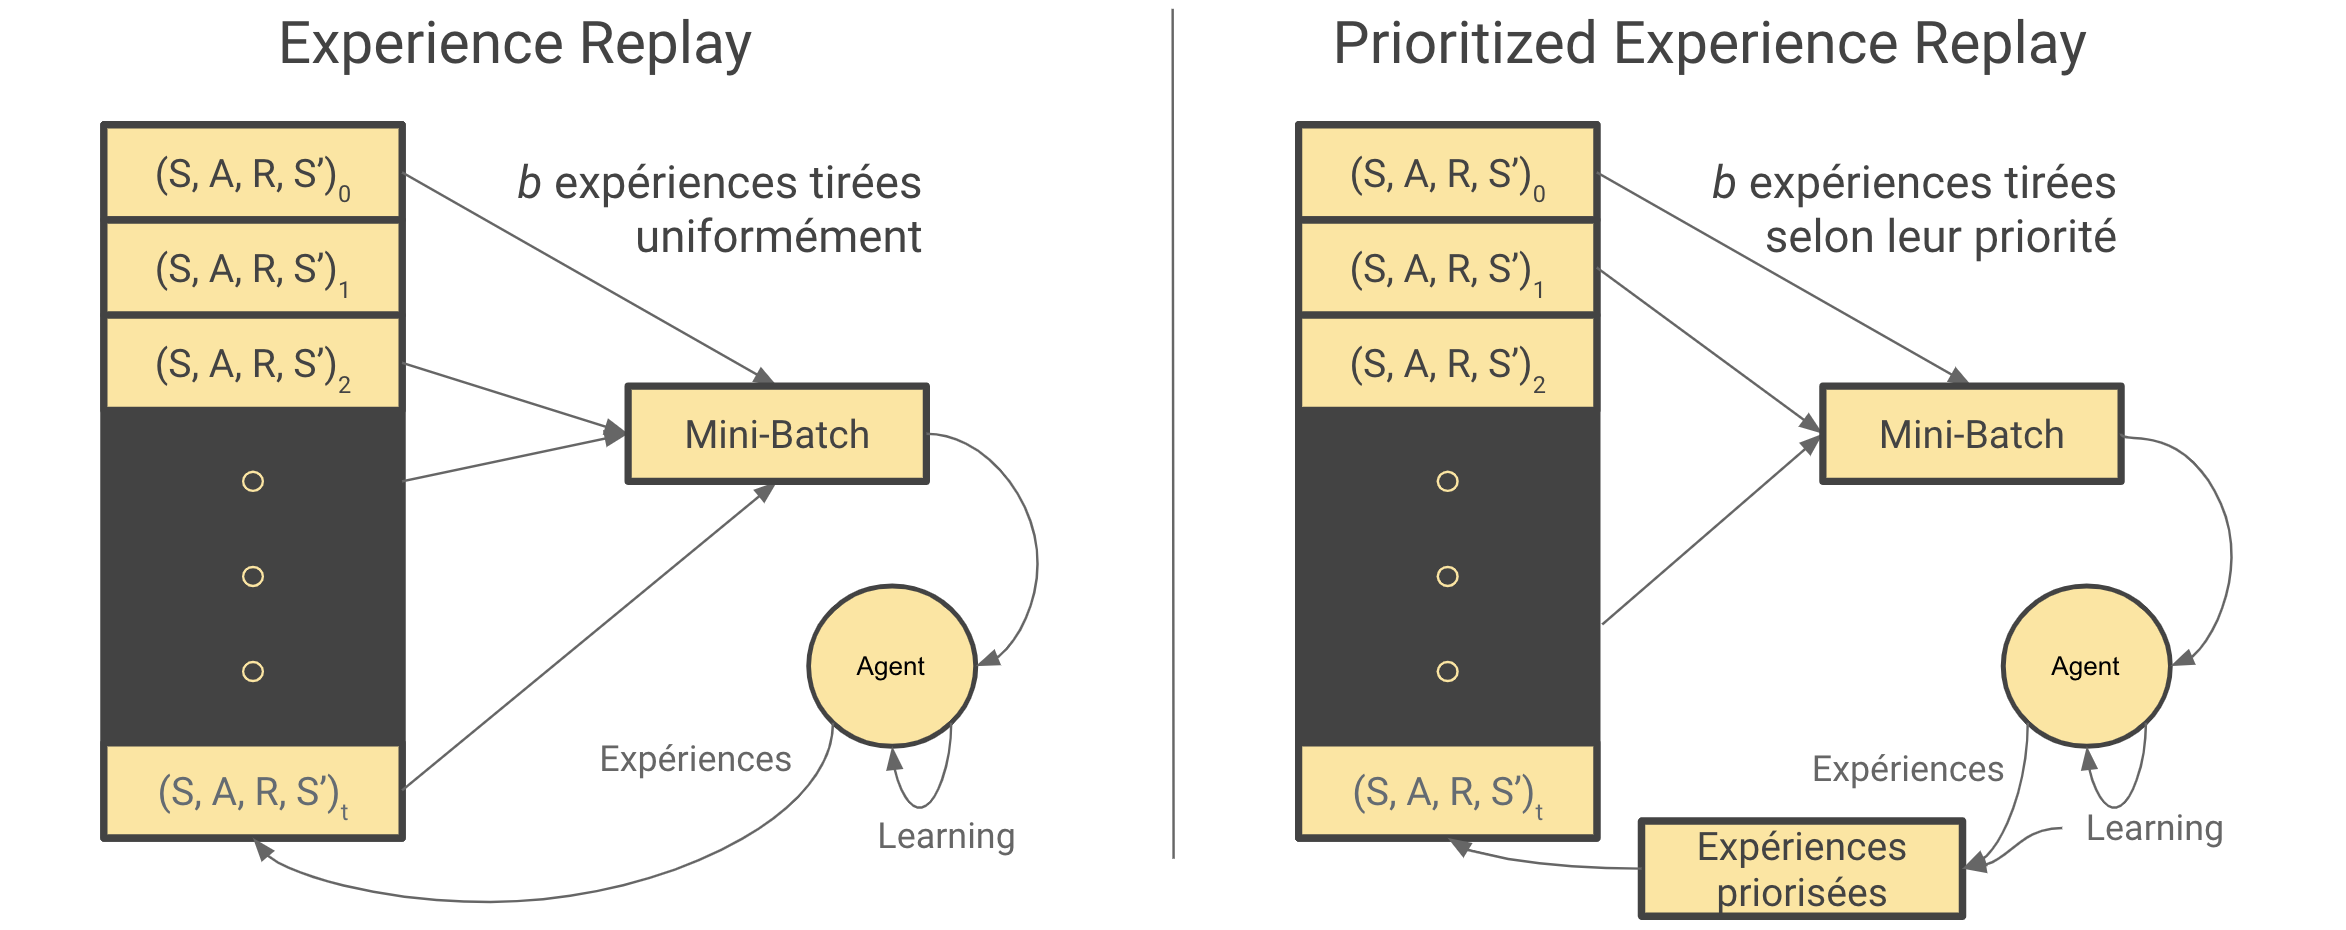
\includegraphics[width=0.80\textwidth]{images/PER.png}
    \captionof{figure}{Vanilla and Prioritized Experience Replay}
    \label{fig:per}
\end{minipage}

\bigbreak

It can be used in training script using the \lstinline[language=bash]+--per+ parameter.
It is for now effective with the DDPG algorithm, but not \textbf{with the TD3}. That is because in the TD3 algorithm there are 2 \textit{Critics} and therefore 2 different TD-Errors from which priorities can be computed. No clear answer has been found in the current literature. We have tried 3 different computation methods:
\begin{itemize}
    \item The \textbf{average} of the 2 TD-Errors
    \item The \textbf{maximum} of the 2 TD-Errors
    \item The TD-Error of the \textit{Critic 1}
\end{itemize}

\section{Wrappers}
To improve the performances of the learning, wrappers can be used to tweak the environment without editing its code.
Wrappers implements the Adapter/Wrapper pattern\footnote{\url{https://en.wikipedia.org/wiki/Adapter_pattern}}.
They are subclasses of gym wrapper classes RewardWrapper, ObservationWrapper and ActionWrapper.
They are instantiated specifying the environment to be wrapped as a constructor parameter.

Let's detail the reward wrapper implementation as an example to review wrappers principle.
The reward wrapper intercepts the result of the step function, and replace the value of reward with a custom reward function.
Figure \ref{fig:rewardwrappers} is a sequence diagram showing how a RewardWrapper interacts with a client class.

ObservationWrapper can be used by overriding the observation(observation) function and ActionWrapper by overriding the action(action) function.
Wrappers contain the original environment as attribute, and can thus access any information from the context.

This section presents the wrappers that have been used for the training of this project.
Wrappers are defined in the \path{learning/utils/wrappers.py} class.

\subsection{Observation Wrappers}
The original state space is $S = \{ 0, 255 \}^{640\times480\times3}$.
This is a very heavy state, especially if we use neural networks to predict the actions from the state.
Thus, the 640x480 pixels are resized to 80x60 pixels and are converted to grayscale images.
This transforms the state space from $S = \{ 0, 255 \}^{640\times480\times3}$ to $S = \{ 0, 255 \}^{80\times60}$.

In order for the robot to have access to information about its speed and acceleration, 4 observations are stacked into a state.
Thus, the state space is now $S = \{ 0, 255 \}^{80\times60\times4}$.

Finally, the observations are normalized to [0, 1], resulting in a $[0, 1]^{80\times60\times4} space$.

\subsection{Reward Wrapper}

% TODO add ref to reward chapter 1
As stated in the first chapter, the original reward function was not really effective during tests.

To try to improve performances, a minimalist reward function has been tested:
\begin{equation}
    R =
    \begin{cases}
        speed, & \text{if}\ dist \leq d\\
        -1, & \text{otherwise}
    \end{cases}
\end{equation}
Where $d$ is a constant defining a minimal distance to the center of the line, over which we consider the robot should be penalised. We used a value $d=0.1\ m$.

The implementation is decoupled from the architecture of actors and critics network, which are defined in \path{actor.py} and \path{critic.py} in the folder \path{learning/reinforcement/pytorch/}.

\section{Architecture}%

\subsection{Actor}%

The Actor's input is a batch of 4 gray-scaled images $80\times80$ (corresponding to what the robot sees at time $t , t-1 , t-2$ and $t-3$) and its output is 2 actions $\in [0,1]^{2}$ for the 2 wheels' velocity.
Then 4 layers are stacked, each one being made of 1 convolutional layer, BatchNorm, and LeakyReLU activation.
Finally 2 fully-connected layers are stacked with a final Sigmoid activation.

\begin{figure}
    \centering
    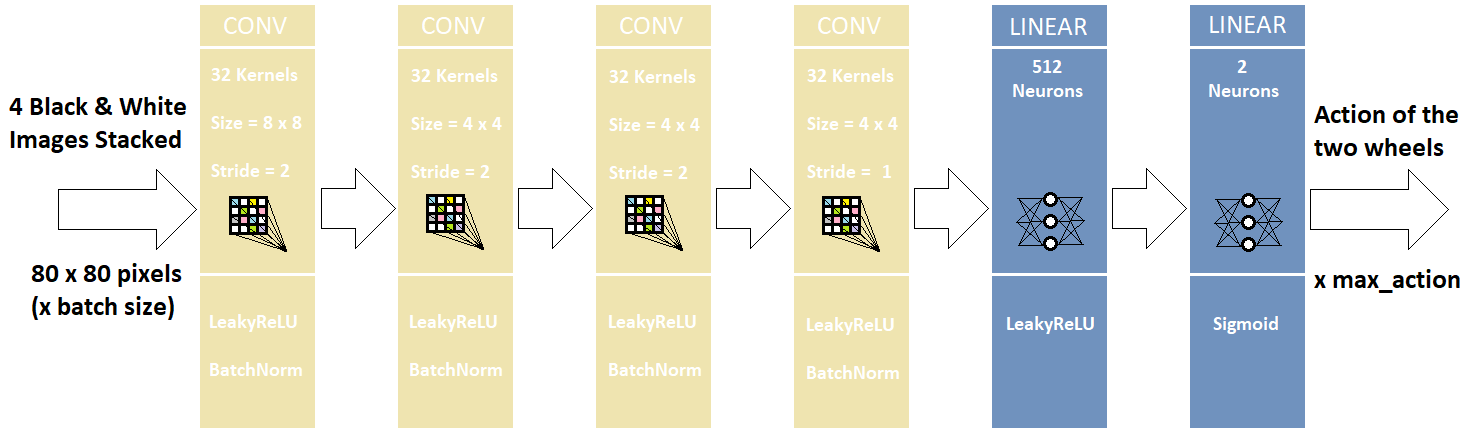
\includegraphics[width=0.80\textwidth]{images/actor_net.png}
    \caption{Actor Architecture}
    \label{actor}
\end{figure}

\subsection{Critic}%

The Critic is really similar to the Actor, except for the last layers. Among the last fully-connected layers, the actions of the two wheels and the hidden outputs are concatenated before the final output of the Actor which is the Q-Value.

\bigbreak

\begin{minipage}{\textwidth}
    \centering
    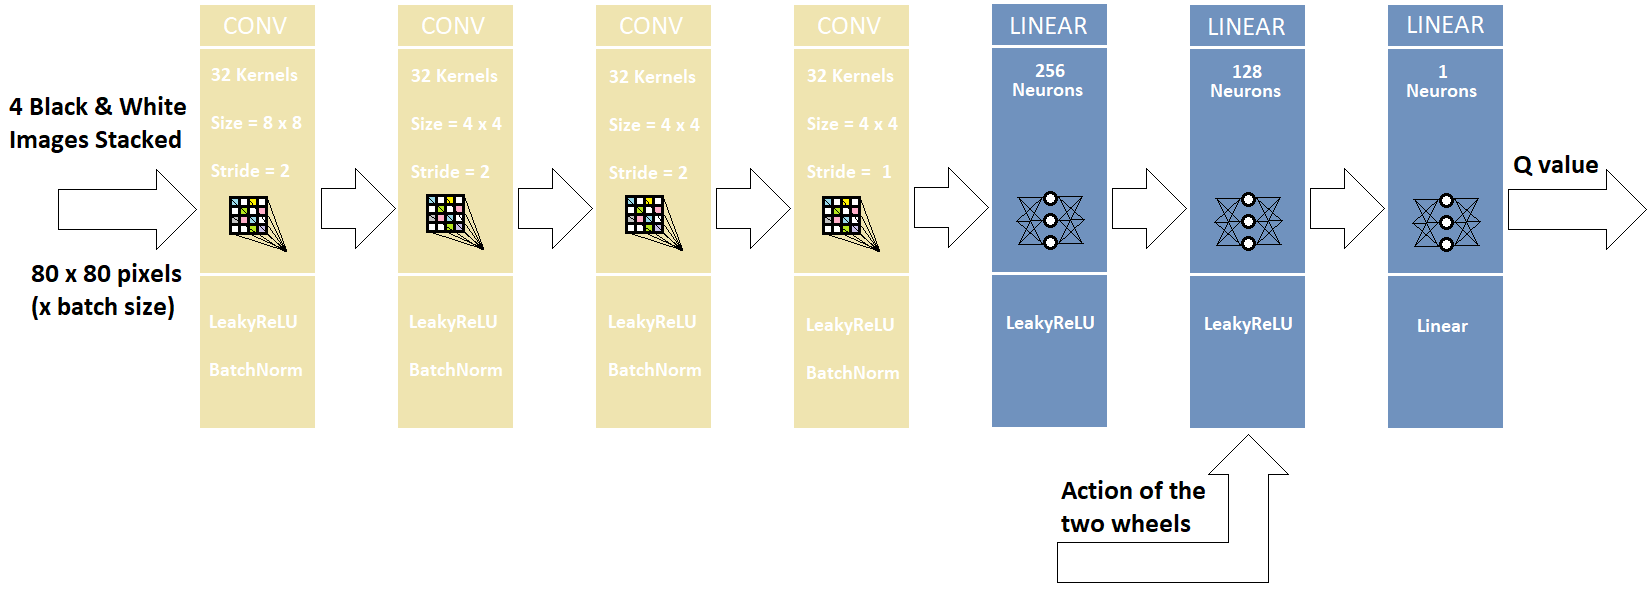
\includegraphics[width=0.80\textwidth]{images/critic_net.png}
    \captionof{figure}{Critic Architecture}
    \label{fig:critic}
\end{minipage}
